\documentclass[a4paper]{article}
\usepackage{ctex}
\usepackage{enumitem}
\usepackage{multirow}
\usepackage{fancyhdr}
\usepackage{float}

\pagestyle{headings}

\setlist[description]{leftmargin=\parindent,labelindent=\parindent}

\begin{document}
\title{简单组合逻辑电路的设计}
\author{梁业升 2019010547(计03)}

\maketitle

\section{实验目的}

\begin{enumerate}
    \item 实现两位加法运算
    \item 实现两位减法运算(显示借位信息,并且当$A<B$时,显示补码表示的差值)
    \item 改进两位减法运算(显示借位信息、计算差的绝对值)
\end{enumerate}

\section{实验原理}

\subsection{两位加法运算}

首先设计1位全加器,电路如下:

\begin{figure}[H]
    \centering
    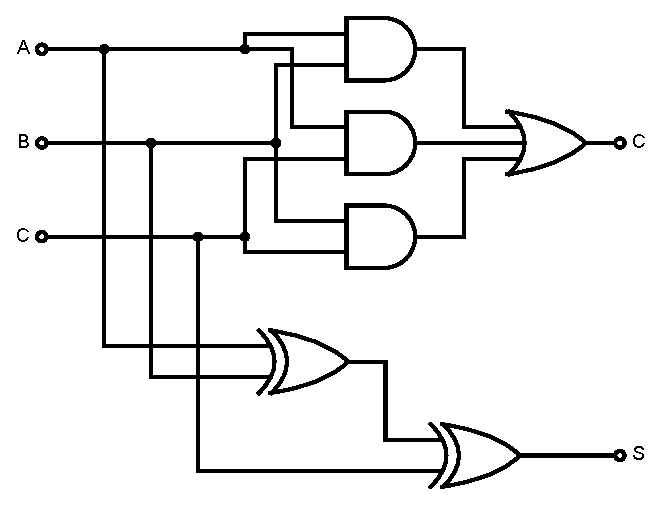
\includegraphics[width=0.5\textwidth]{./assets/1-bit.eps}
    \caption{1位全加器}
\end{figure}

将1位全加器级联,得到两位全加器:

\begin{figure}[H]
    \centering
    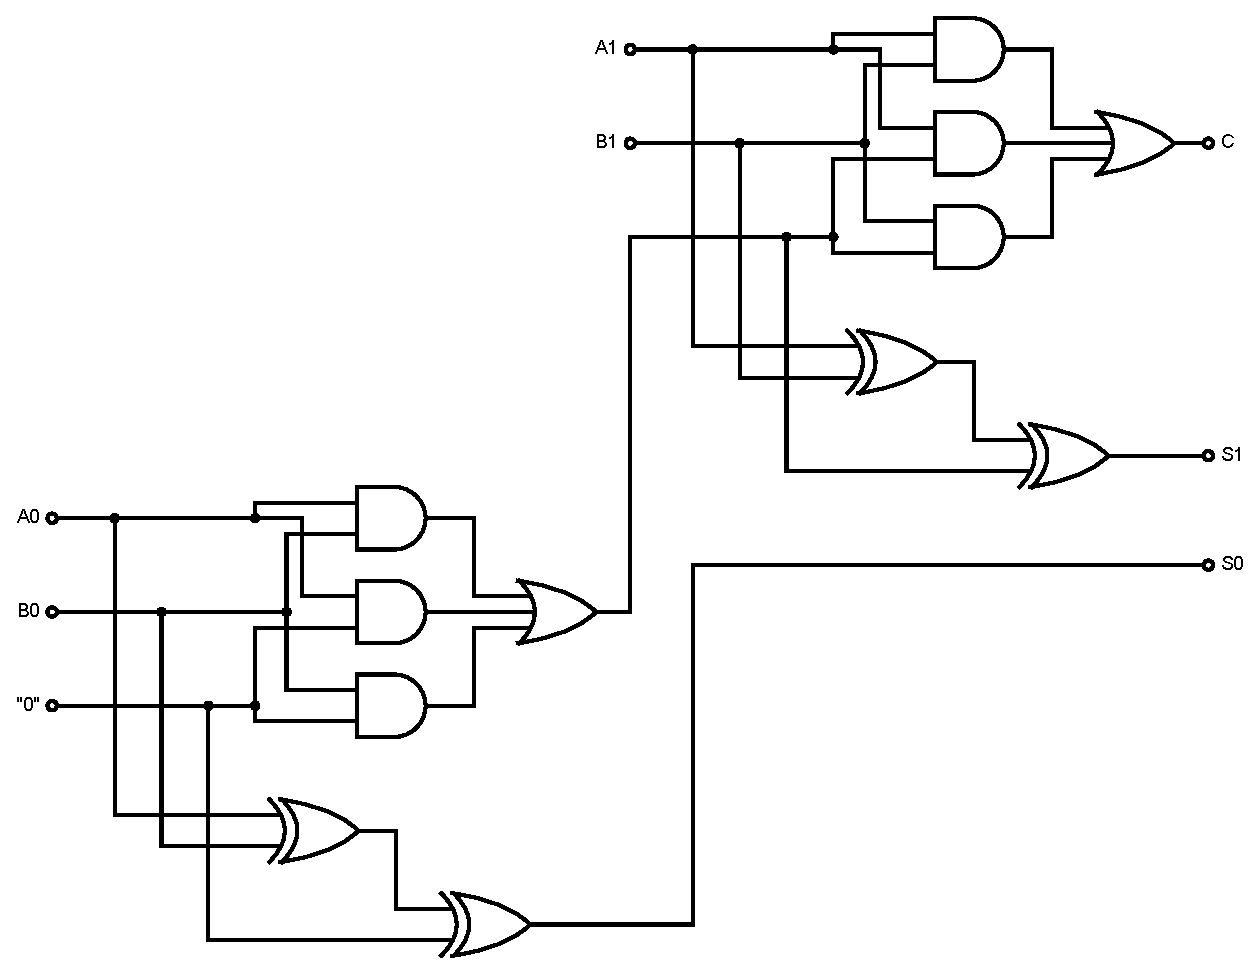
\includegraphics[width=0.8\textwidth]{./assets/2-bit.eps}
    \caption{2位全加器}
\end{figure}

\subsection{两位减法运算}

在2位加法器的基础上,对被减数“取反、加1”,并对输出的进位信号取反,即可得到2位减法器:

\begin{figure}[H]
    \centering
    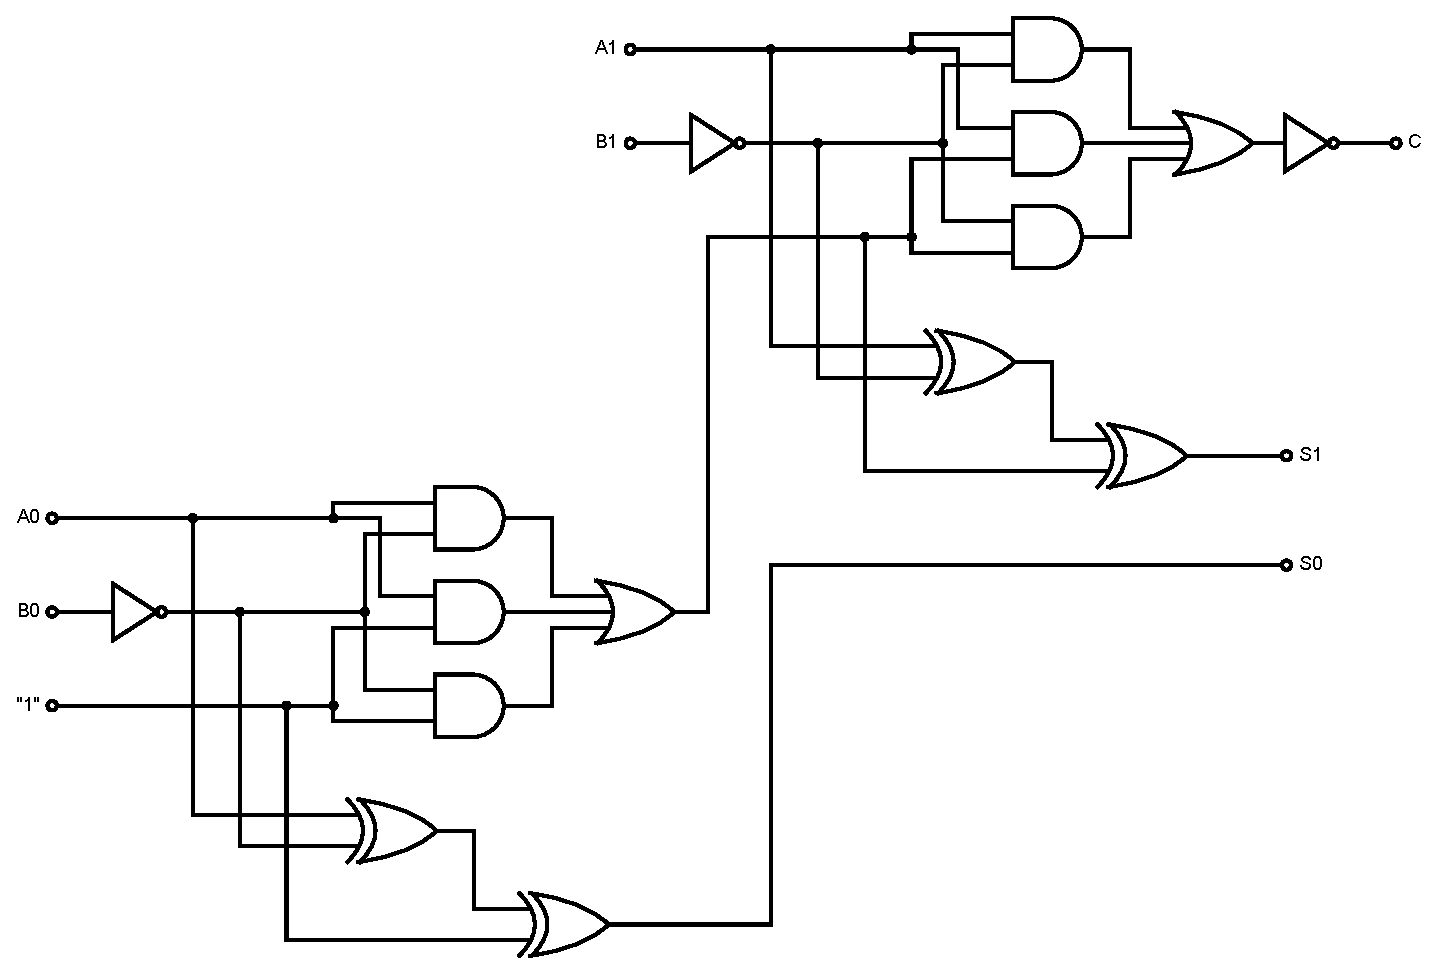
\includegraphics[width=0.9\textwidth]{./assets/2-bit-sub.eps}
    \caption{2位减法器}
\end{figure}

\subsection{改进的两位减法运算}

根据2位减法器的借位信息$C$,若$C$为1则输出原码:

\begin{figure}[H]
    \centering
    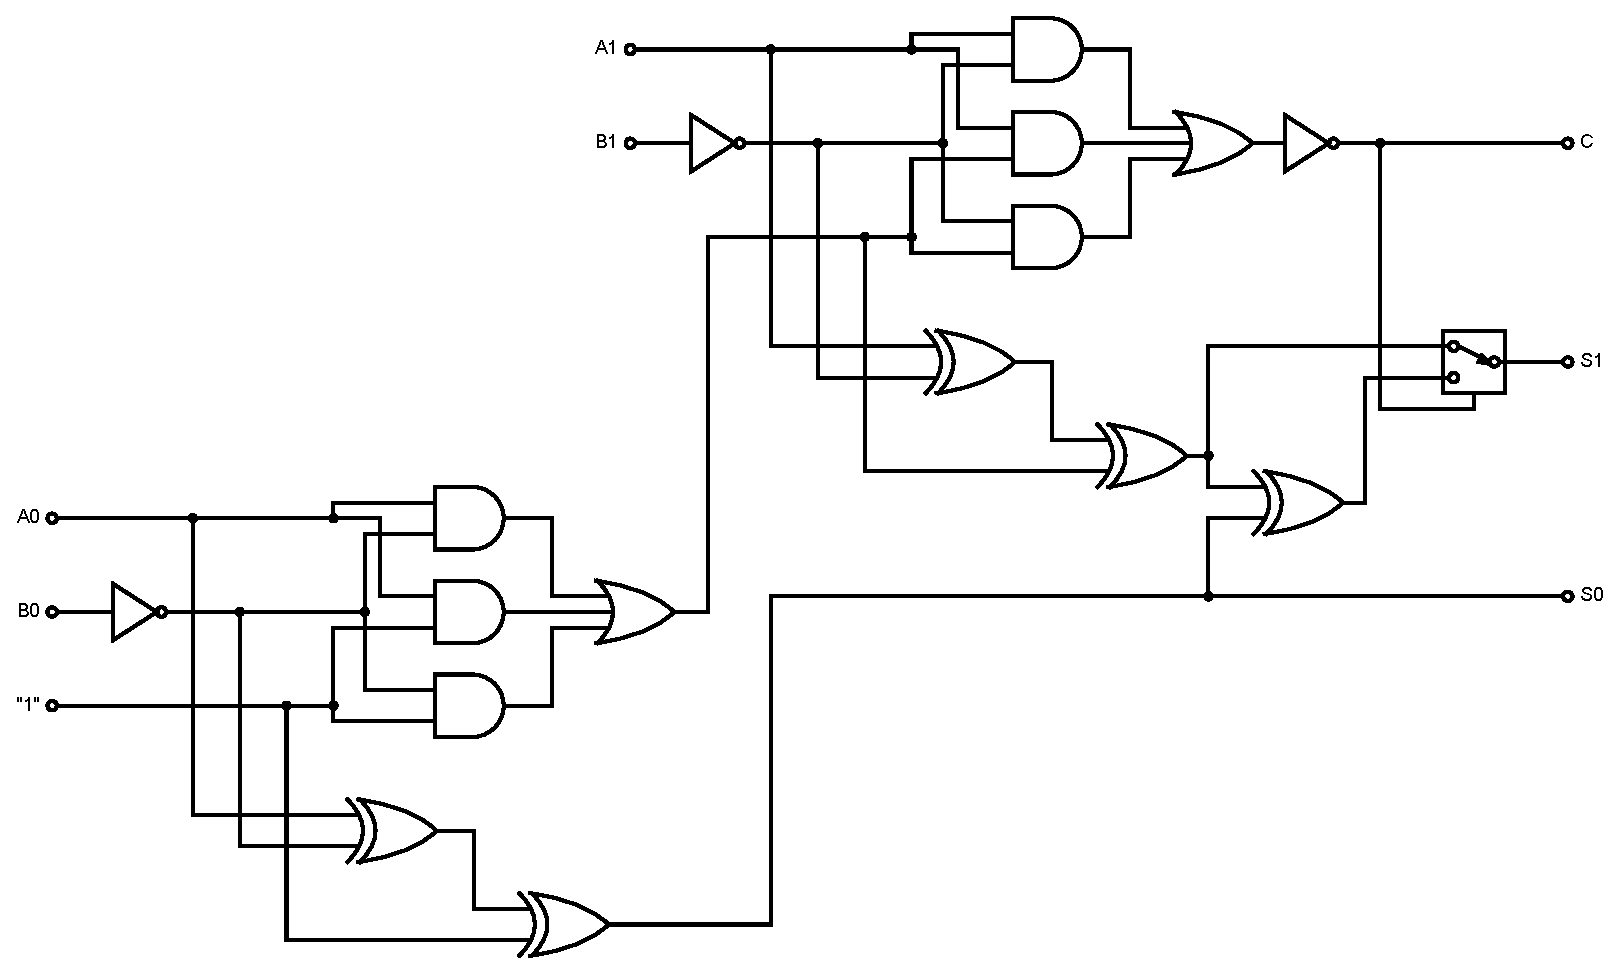
\includegraphics[width=0.9\textwidth]{./assets/2-bit-sub-advanced.eps}
    \caption{改进的2位减法器}
\end{figure}

\section{思考题}

设计一个4位二进制除法运算电路,A为被除数,B为除数,C为商,D为余数。

\begin{figure}[H]
    \centering
    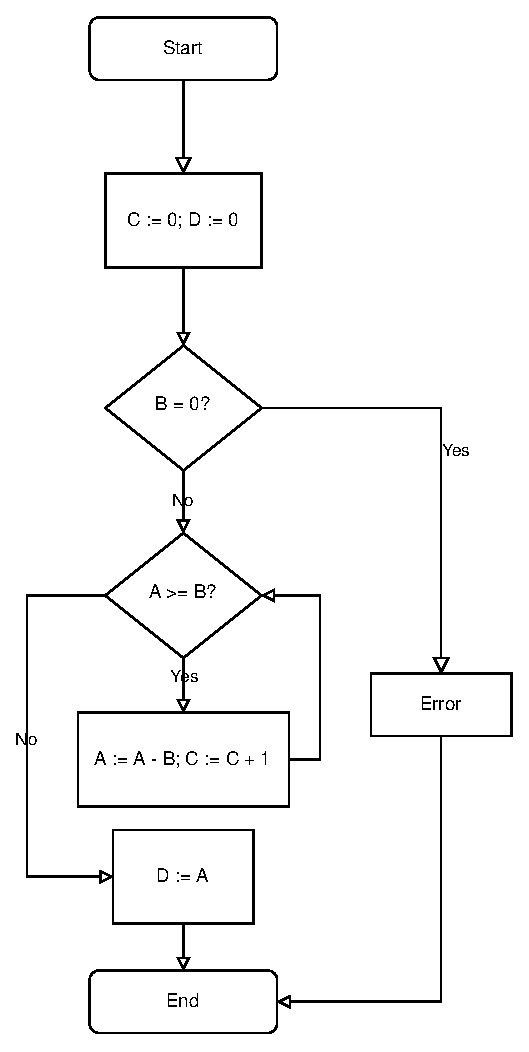
\includegraphics[width=0.5\textwidth]{./assets/flow.eps}
    \caption{除法器流程图}
\end{figure}

\begin{enumerate}
    \item 首先判断被除数是否合法
    \item 当被除数大于除数时,从被除数中减去除数,商加1,并重复此过程
    \item 直到被除数小于除数时,将被除数赋值给余数
\end{enumerate}

\end{document}
